% Slide 3: Compile -> Upload -> Start pipeline.
%
% Four-panel horizontal flow:
%   1. Python source                        [ compile ] ->
%   2. IR stack (arrus L1, us4r/gpu L2, device asm/kernels)
%                                            [ upload ] ->
%   3. Device memory: code memory + variable memory (side by side)
%                                            [ start ] ->
%   4. Running ultrasound system (frames + processing + display, looping)
%
% Colors match ndarray_common.tex conventions:
%   green  = CPU/host (Python source)
%   orange = GPU dialect / GPU kernels
%   teal   = ultrasound device / us4r
%   gold   = variables
%   gray   = device asm
%
% Build: pdflatex slide3_compile_upload_run.tex

\documentclass[tikz,border=6pt]{standalone}
% Shared preamble for NdArray graph figures.
% Include with: % Shared preamble for NdArray graph figures.
% Include with: % Shared preamble for NdArray graph figures.
% Include with: \input{ndarray_common}
%
% Provides a consistent color palette and node styles for the three figures
% in docs/td/ndarray_design.md.

\usepackage{tikz}
\usetikzlibrary{positioning, arrows.meta, fit, calc, backgrounds, shapes.geometric}

% --- Device / role color palette ------------------------------------------------
\definecolor{arrusUs4R}   {HTML}{2CA9BC}   % ultrasound device (teal)
\definecolor{arrusGPU}    {HTML}{F28C28}   % CUDA GPU (orange)
\definecolor{arrusCPU}    {HTML}{4CAF50}   % CPU (green)
\definecolor{arrusHost}   {HTML}{9E9E9E}   % host / control (gray)
\definecolor{arrusBuffer} {HTML}{616161}   % stream buffer (dark gray)
\definecolor{arrusVariable}{HTML}{F4C542}  % Variable (gold)
\definecolor{arrusTrigger}{HTML}{D64545}   % Trigger source (red)
\definecolor{arrusOutput} {HTML}{5C6BC0}   % Graph output / sink (indigo)

% --- Node styles ---------------------------------------------------------------
\tikzset{
  op/.style       = {rectangle, rounded corners=2pt, draw=black!60, thick,
                     minimum width=26mm, minimum height=8mm, align=center,
                     font=\small},
  op/us4r/.style  = {op, fill=arrusUs4R!25,   draw=arrusUs4R!80!black},
  op/gpu/.style   = {op, fill=arrusGPU!25,    draw=arrusGPU!80!black},
  op/cpu/.style   = {op, fill=arrusCPU!25,    draw=arrusCPU!70!black},
  op/host/.style  = {op, fill=arrusHost!20,   draw=arrusHost!70!black},
  op/output/.style= {op, fill=arrusOutput!25, draw=arrusOutput!80!black},
  op/variable/.style = {ellipse, draw=arrusVariable!70!black, thick,
                        fill=arrusVariable!30, minimum width=22mm,
                        minimum height=7mm, align=center, font=\small\itshape},
  op/trigger/.style  = {regular polygon, regular polygon sides=3,
                        draw=arrusTrigger!80!black, thick, fill=arrusTrigger!25,
                        minimum size=11mm, align=center, font=\scriptsize,
                        inner sep=0pt},
  op/buffer/.style   = {cylinder, shape border rotate=90, aspect=0.3,
                        draw=arrusBuffer!80!black, thick, fill=arrusBuffer!15,
                        minimum width=18mm, minimum height=10mm, align=center,
                        font=\scriptsize},
  edge/.style        = {-{Latex[length=2mm]}, thick, draw=black!70},
  % Intra-region data flow: shared buffer + CUDA-stream / kernel-order
  % ordering. No runtime queue.
  edge/intra/.style  = {-{Latex[length=2mm]}, thick, draw=black!70},
  % Cross-region stream: real queue infrastructure (backpressure/drop policy,
  % scheduler wake-up). Used for cross-device transfers and rate mismatches.
  edge/stream/.style = {-{Latex[length=2mm]}, very thick, draw=black!70,
                        double distance=1pt},
  edge/trigger/.style= {-{Latex[length=2mm]}, thick, draw=arrusTrigger!80!black,
                        dashed},
  edge/variable/.style = {-{Latex[length=2mm]}, thick,
                          draw=arrusVariable!80!black, densely dotted},
  region/.style      = {rounded corners, inner sep=4mm, dashed,
                        line width=0.8pt},
  region/us4r/.style = {region, draw=arrusUs4R!70!black, fill=arrusUs4R!5},
  region/gpu/.style  = {region, draw=arrusGPU!70!black,  fill=arrusGPU!5},
  legendbox/.style   = {rectangle, draw=black!30, rounded corners=2pt,
                        inner sep=4pt, fill=white},
}

%
% Provides a consistent color palette and node styles for the three figures
% in docs/td/ndarray_design.md.

\usepackage{tikz}
\usetikzlibrary{positioning, arrows.meta, fit, calc, backgrounds, shapes.geometric}

% --- Device / role color palette ------------------------------------------------
\definecolor{arrusUs4R}   {HTML}{2CA9BC}   % ultrasound device (teal)
\definecolor{arrusGPU}    {HTML}{F28C28}   % CUDA GPU (orange)
\definecolor{arrusCPU}    {HTML}{4CAF50}   % CPU (green)
\definecolor{arrusHost}   {HTML}{9E9E9E}   % host / control (gray)
\definecolor{arrusBuffer} {HTML}{616161}   % stream buffer (dark gray)
\definecolor{arrusVariable}{HTML}{F4C542}  % Variable (gold)
\definecolor{arrusTrigger}{HTML}{D64545}   % Trigger source (red)
\definecolor{arrusOutput} {HTML}{5C6BC0}   % Graph output / sink (indigo)

% --- Node styles ---------------------------------------------------------------
\tikzset{
  op/.style       = {rectangle, rounded corners=2pt, draw=black!60, thick,
                     minimum width=26mm, minimum height=8mm, align=center,
                     font=\small},
  op/us4r/.style  = {op, fill=arrusUs4R!25,   draw=arrusUs4R!80!black},
  op/gpu/.style   = {op, fill=arrusGPU!25,    draw=arrusGPU!80!black},
  op/cpu/.style   = {op, fill=arrusCPU!25,    draw=arrusCPU!70!black},
  op/host/.style  = {op, fill=arrusHost!20,   draw=arrusHost!70!black},
  op/output/.style= {op, fill=arrusOutput!25, draw=arrusOutput!80!black},
  op/variable/.style = {ellipse, draw=arrusVariable!70!black, thick,
                        fill=arrusVariable!30, minimum width=22mm,
                        minimum height=7mm, align=center, font=\small\itshape},
  op/trigger/.style  = {regular polygon, regular polygon sides=3,
                        draw=arrusTrigger!80!black, thick, fill=arrusTrigger!25,
                        minimum size=11mm, align=center, font=\scriptsize,
                        inner sep=0pt},
  op/buffer/.style   = {cylinder, shape border rotate=90, aspect=0.3,
                        draw=arrusBuffer!80!black, thick, fill=arrusBuffer!15,
                        minimum width=18mm, minimum height=10mm, align=center,
                        font=\scriptsize},
  edge/.style        = {-{Latex[length=2mm]}, thick, draw=black!70},
  % Intra-region data flow: shared buffer + CUDA-stream / kernel-order
  % ordering. No runtime queue.
  edge/intra/.style  = {-{Latex[length=2mm]}, thick, draw=black!70},
  % Cross-region stream: real queue infrastructure (backpressure/drop policy,
  % scheduler wake-up). Used for cross-device transfers and rate mismatches.
  edge/stream/.style = {-{Latex[length=2mm]}, very thick, draw=black!70,
                        double distance=1pt},
  edge/trigger/.style= {-{Latex[length=2mm]}, thick, draw=arrusTrigger!80!black,
                        dashed},
  edge/variable/.style = {-{Latex[length=2mm]}, thick,
                          draw=arrusVariable!80!black, densely dotted},
  region/.style      = {rounded corners, inner sep=4mm, dashed,
                        line width=0.8pt},
  region/us4r/.style = {region, draw=arrusUs4R!70!black, fill=arrusUs4R!5},
  region/gpu/.style  = {region, draw=arrusGPU!70!black,  fill=arrusGPU!5},
  legendbox/.style   = {rectangle, draw=black!30, rounded corners=2pt,
                        inner sep=4pt, fill=white},
}

%
% Provides a consistent color palette and node styles for the three figures
% in docs/td/ndarray_design.md.

\usepackage{tikz}
\usetikzlibrary{positioning, arrows.meta, fit, calc, backgrounds, shapes.geometric}

% --- Device / role color palette ------------------------------------------------
\definecolor{arrusUs4R}   {HTML}{2CA9BC}   % ultrasound device (teal)
\definecolor{arrusGPU}    {HTML}{F28C28}   % CUDA GPU (orange)
\definecolor{arrusCPU}    {HTML}{4CAF50}   % CPU (green)
\definecolor{arrusHost}   {HTML}{9E9E9E}   % host / control (gray)
\definecolor{arrusBuffer} {HTML}{616161}   % stream buffer (dark gray)
\definecolor{arrusVariable}{HTML}{F4C542}  % Variable (gold)
\definecolor{arrusTrigger}{HTML}{D64545}   % Trigger source (red)
\definecolor{arrusOutput} {HTML}{5C6BC0}   % Graph output / sink (indigo)

% --- Node styles ---------------------------------------------------------------
\tikzset{
  op/.style       = {rectangle, rounded corners=2pt, draw=black!60, thick,
                     minimum width=26mm, minimum height=8mm, align=center,
                     font=\small},
  op/us4r/.style  = {op, fill=arrusUs4R!25,   draw=arrusUs4R!80!black},
  op/gpu/.style   = {op, fill=arrusGPU!25,    draw=arrusGPU!80!black},
  op/cpu/.style   = {op, fill=arrusCPU!25,    draw=arrusCPU!70!black},
  op/host/.style  = {op, fill=arrusHost!20,   draw=arrusHost!70!black},
  op/output/.style= {op, fill=arrusOutput!25, draw=arrusOutput!80!black},
  op/variable/.style = {ellipse, draw=arrusVariable!70!black, thick,
                        fill=arrusVariable!30, minimum width=22mm,
                        minimum height=7mm, align=center, font=\small\itshape},
  op/trigger/.style  = {regular polygon, regular polygon sides=3,
                        draw=arrusTrigger!80!black, thick, fill=arrusTrigger!25,
                        minimum size=11mm, align=center, font=\scriptsize,
                        inner sep=0pt},
  op/buffer/.style   = {cylinder, shape border rotate=90, aspect=0.3,
                        draw=arrusBuffer!80!black, thick, fill=arrusBuffer!15,
                        minimum width=18mm, minimum height=10mm, align=center,
                        font=\scriptsize},
  edge/.style        = {-{Latex[length=2mm]}, thick, draw=black!70},
  % Intra-region data flow: shared buffer + CUDA-stream / kernel-order
  % ordering. No runtime queue.
  edge/intra/.style  = {-{Latex[length=2mm]}, thick, draw=black!70},
  % Cross-region stream: real queue infrastructure (backpressure/drop policy,
  % scheduler wake-up). Used for cross-device transfers and rate mismatches.
  edge/stream/.style = {-{Latex[length=2mm]}, very thick, draw=black!70,
                        double distance=1pt},
  edge/trigger/.style= {-{Latex[length=2mm]}, thick, draw=arrusTrigger!80!black,
                        dashed},
  edge/variable/.style = {-{Latex[length=2mm]}, thick,
                          draw=arrusVariable!80!black, densely dotted},
  region/.style      = {rounded corners, inner sep=4mm, dashed,
                        line width=0.8pt},
  region/us4r/.style = {region, draw=arrusUs4R!70!black, fill=arrusUs4R!5},
  region/gpu/.style  = {region, draw=arrusGPU!70!black,  fill=arrusGPU!5},
  legendbox/.style   = {rectangle, draw=black!30, rounded corners=2pt,
                        inner sep=4pt, fill=white},
}

\usetikzlibrary{decorations.pathmorphing}

\begin{document}
\begin{tikzpicture}[
    node distance=6mm and 22mm,
    every node/.append style={font=\small},
    panel/.style     = {rectangle, rounded corners=4pt, thick, align=left,
                        inner sep=8pt, text width=56mm},
    tier/.style      = {rectangle, rounded corners=2pt, thick, align=left,
                        text width=48mm, inner sep=5pt,
                        font=\ttfamily\scriptsize},
    arrow/.style     = {-{Latex[length=4mm]}, ultra thick, draw=black!65},
    phase/.style     = {font=\Large\bfseries, text=black!80, align=center,
                        fill=white, inner sep=3pt},
]

  % ==========================================================================
  % Panel 1 --- Python source
  % ==========================================================================
  \node[panel, draw=arrusCPU!80!black, fill=arrusCPU!5]
       (py) at (0,0)
    {\textbf{\normalsize Python source}\\[6pt]
     \begin{tikzpicture}
       \node[tier, draw=arrusCPU!70!black, fill=arrusCPU!15] {%
         import arrus.numpy as anp\\
         ~\\
         with arrus.Graph() as g:\\
         ~~f\phantom{xx} = anp.tx\_rx\_seq(@indices)\\
         ~~b\phantom{xx} = anp.beamform(f)\\
         ~~img = anp.scan\_convert(b)\\
         ~\\
         session.compile(g)\\
         session.upload()\\
         session.start()
       };
     \end{tikzpicture}
    };

  % ==========================================================================
  % Panel 2 --- IR stack (three tiers + pruning symbol at bottom)
  % ==========================================================================
  \node[panel, right=32mm of py, draw=black!50, fill=black!2]
       (ir)
    {\textbf{\normalsize IR stack}\\[6pt]
     \begin{tikzpicture}[node distance=3mm]
       \node[tier, draw=arrusGPU!70!black, fill=arrusGPU!15] (l1) {%
         {\bfseries Level 1 --- arrus dialect}\\
         f\phantom{xx}\ = arrus.tx\_rx\_seq(@indices)\\
         b\phantom{xx}\ = arrus.beamform(f)\\
         img = arrus.scan\_convert(b)
       };
       \node[tier, draw=arrusUs4R!70!black, fill=arrusUs4R!15, below=of l1] (l2) {%
         {\bfseries Level 2 --- us4r + gpu}\\
         w = us4r.rebind\_wiring(@indices)\\
         f = us4r.fire\_sequence(w)\\
         b = gpu.beamform(f)
       };
       % --- Graph pruning visual: before/after mini graphs ---
       % (IR-level optimization; sits between L2 and device asm)
       \node[tier, draw=arrusTrigger!60!black, fill=arrusTrigger!8,
             below=of l2, text width=48mm, inner sep=4pt] (prune) {%
         {\bfseries\scriptsize + graph pruning / DCE / canonicalization}\\[2pt]
         \begin{tikzpicture}[node distance=0mm, baseline=(before.center)]
           % Before graph (5 nodes, some dead)
           \node[circle, draw=black!60, fill=black!10, minimum size=2.5mm,
                 inner sep=0] (b0) at (0,0)   {};
           \node[circle, draw=black!60, fill=black!10, minimum size=2.5mm,
                 inner sep=0] (b1) at (5mm,3mm) {};
           \node[circle, draw=black!60, fill=black!10, minimum size=2.5mm,
                 inner sep=0] (b2) at (10mm,0) {};
           \node[circle, draw=black!35, fill=black!5, minimum size=2.5mm,
                 inner sep=0, dashed] (b3) at (5mm,-3mm) {};
           \node[circle, draw=black!35, fill=black!5, minimum size=2.5mm,
                 inner sep=0, dashed] (b4) at (12mm,3.5mm) {};
           \draw[thin, black!55]  (b0)--(b1) (b1)--(b2);
           \draw[thin, black!30, dashed] (b0)--(b3) (b1)--(b4);
           % Label
           \node[below=0.5mm of b3, font=\tiny\itshape,
                 text=black!55, xshift=-2mm] (before) {before};

           % Prune arrow
           \node[right=1.5mm of b4, font=\tiny\bfseries,
                 text=arrusTrigger!70!black] (parrow) {$\Rightarrow$};

           % After graph (3 nodes only)
           \node[circle, draw=arrusGPU!80!black, fill=arrusGPU!30,
                 minimum size=2.5mm, inner sep=0]
                (a0) at ($(parrow.east)+(3mm,-1.5mm)$) {};
           \node[circle, draw=arrusGPU!80!black, fill=arrusGPU!30,
                 minimum size=2.5mm, inner sep=0]
                (a1) at ($(a0)+(5mm,3mm)$) {};
           \node[circle, draw=arrusGPU!80!black, fill=arrusGPU!30,
                 minimum size=2.5mm, inner sep=0]
                (a2) at ($(a1)+(5mm,-3mm)$) {};
           \draw[thin, black!55] (a0)--(a1) (a1)--(a2);
           \node[below=0.5mm of a1, font=\tiny\itshape,
                 text=black!55, yshift=-3mm] {after};
         \end{tikzpicture}
       };
       \node[tier, draw=black!45, fill=black!8, below=of prune] (asm) {%
         {\bfseries Device asm / kernels}\\
         us4r: TX[i]\{ap, dl, pl\}\\
         DMA descriptors [0..K]\\
         GPU PTX / SASS
       };
     \end{tikzpicture}
    };

  % ==========================================================================
  % Panel 3 --- Device memory (code + variables)
  % ==========================================================================
  \node[panel, right=32mm of ir, draw=black!50, fill=black!2]
       (mem)
    {\textbf{\normalsize Device memory}\\[6pt]
     \begin{tikzpicture}[node distance=3mm]
       \node[tier, draw=arrusUs4R!70!black, fill=arrusUs4R!15] (codemem) {%
         {\bfseries Code memory}\\
         TX/RX linked list [0..191]\\
         GPU kernels loaded\\
         DMA descriptor table
       };
       \node[tier, draw=arrusVariable!70!black, fill=arrusVariable!25,
             below=of codemem] (varmem) {%
         {\bfseries Variable memory}\\
         @indices = [3, 5, 8, 13, \ldots]\\
         @sos\phantom{xxxx} = 1540.0\\
         @tgc\phantom{xxxx} = [\ldots]
       };
     \end{tikzpicture}
    };

  % ==========================================================================
  % Panel 4 --- Physical running ultrasound system
  % Simple stylized drawing: monitor on stand + coiled cable + probe.
  % ==========================================================================
  \node[panel, right=32mm of mem, draw=arrusUs4R!80!black, fill=arrusUs4R!8]
       (run)
    {\textbf{\normalsize Running system}\\[6pt]
     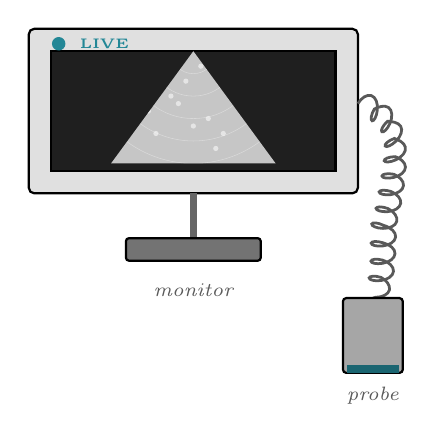
\begin{tikzpicture}[scale=0.95]
       % --- Monitor bezel ---
       \draw[thick, rounded corners=2pt, fill=black!12]
         (-22mm,0) rectangle (22mm,22mm);
       % Screen (dark inner rectangle)
       \draw[thick, fill=black!88]
         (-19mm,3mm) rectangle (19mm,19mm);
       % B-mode sector: fan shape with concentric depth arcs + speckles
       \begin{scope}
         \clip (0,19mm) -- (-11mm,4mm) -- (11mm,4mm) -- cycle;
         \fill[gray!45] (-19mm,3mm) rectangle (19mm,19mm);
         \foreach \r in {3,6,9,12,15} {
           \draw[white, opacity=0.35, very thin] (0,19mm) circle (\r mm);
         }
         % A few speckles suggesting tissue texture
         \foreach \x/\y in {-3/13, 2/10, 4/15, -5/8, 1/17, 3/6,
                            -2/12, 5/14, -6/11, 0/9, 4/8, -1/15} {
           \fill[white, opacity=0.55] (\x mm, \y mm) circle (0.35mm);
         }
       \end{scope}

       % --- Monitor stand + base ---
       \draw[line width=2.5pt, black!60] (0,0) -- (0,-6mm);
       \draw[thick, fill=black!55, rounded corners=1pt]
         (-9mm,-9mm) rectangle (9mm,-6mm);

       % --- Coiled cable from right side of monitor to probe ---
       \draw[line width=1pt, black!65, decorate,
             decoration={coil, aspect=0.5, segment length=2.2mm,
                         amplitude=1.5mm}]
         (22mm,12mm) .. controls +(6mm,-2mm) and +(1mm,6mm) .. (26mm,-2mm)
                     .. controls +(-1mm,-4mm) and +(2mm,4mm) .. (24mm,-14mm);

       % --- Probe ---
       \draw[thick, fill=black!35, rounded corners=1.2pt]
         (20mm,-24mm) rectangle (28mm,-14mm);
       % Probe transducer face (thin lighter strip at the bottom)
       \fill[arrusUs4R!60!black] (20.5mm,-24mm) rectangle (27.5mm,-23mm);

       % --- Labels ---
       \node[font=\scriptsize\itshape, text=black!65] at (0,-13mm) {monitor};
       \node[font=\scriptsize\itshape, text=black!65] at (24mm,-27mm) {probe};

       % --- Live-scanning indicator ---
       \fill[arrusUs4R!80!black] (-18mm,20mm) circle (0.9mm);
       \node[right=0.5mm, font=\tiny\bfseries, text=arrusUs4R!80!black]
         at (-17mm,20mm) {LIVE};
     \end{tikzpicture}
    };

  % ==========================================================================
  % Phase arrows between panels
  % ==========================================================================
  \draw[arrow] (py.east)  -- (ir.west);
  \node[phase] at ($(py.east)!0.5!(ir.west)$) {[ compile ]};

  \draw[arrow] (ir.east)  -- (mem.west);
  \node[phase] at ($(ir.east)!0.5!(mem.west)$) {[ upload ]};

  \draw[arrow] (mem.east) -- (run.west);
  \node[phase] at ($(mem.east)!0.5!(run.west)$) {[ start ]};

\end{tikzpicture}
\end{document}
